\documentclass{beamer}

\usepackage[default]{lato}
\usepackage{inconsolata}
\usepackage{fontawesome}
\usepackage[orientation=landscape,size=a1,scale=1]{beamerposter}
\usepackage{graphicx}
\usepackage{tcolorbox}
\usepackage{tikz}

\definecolor{myblue}{RGB}{0, 164, 216}
\definecolor{mygrey}{RGB}{63, 63, 63}

\tcbset{%
    noparskip,
    colback=gray!10, %background color of the box
    colframe=gray!30, %color of frame and title background
    coltext=mygrey, %color of body text
    coltitle=mygrey, %color of title text 
    fonttitle=\bfseries,
}

\begin{document}

\color{mygrey}
%%% TITLE %%%

\begin{columns}
    \begin{column}{0.1\textwidth}
        \vspace{2em}

        \centering%
        
\includegraphics[width=\linewidth]{img/cu_logo}
    \end{column}

    \begin{column}{0.75\textwidth}
        \vspace{2em}

        \centering%
        {%
            \fontsize{60}{72}\selectfont%
            Evolutionary dataset optimisation:\vspace{.5ex}
            learning algorithm quality through evolution
        }
    \end{column}

    \begin{column}{0.1\textwidth}
        \vspace{2em}

        \centering%
        
\includegraphics[width=\linewidth]{img/paper_qr}
    \end{column}
\end{columns}

\vspace{3em}

%%% MAIN BODY %%%

\begin{columns}
    \begin{column}{0.6\textwidth}
    \begin{tcolorbox}%[title=\huge{The evolutionary algorithm}]

    \Huge{\textbf{\textcolor{myblue}{The evolutionary algorithm}}}
    \huge{}

    \begin{tikzpicture}

    \node (ind) at (0, 0) {%
        \begin{tabular}{c}
            \huge{Create individuals}\vspace{.5ex}\\
            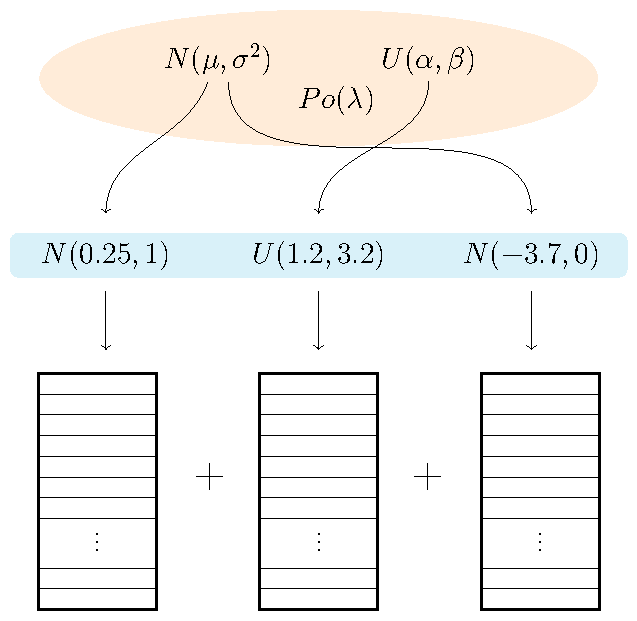
\includegraphics[width=.25\textwidth]{tex/individual.pdf}
        \end{tabular}
        };

    \node (sel) at (5, -22){%
        \begin{tabular}{c}
            \huge{Select parents}\vspace{.5ex}\\
            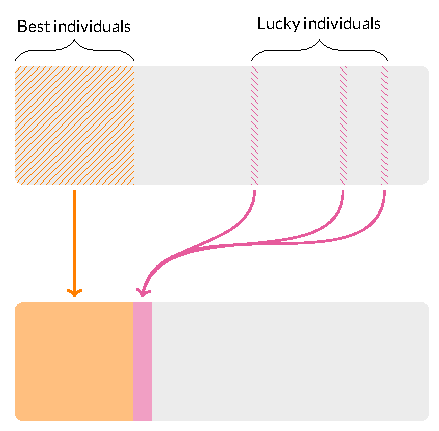
\includegraphics[width=.25\textwidth]{tex/selection.pdf}
        \end{tabular}
    };

    \node (cro) at (25, 0) {%
        \begin{tabular}{c}
            \huge{Create offspring}\vspace{.5ex}\\
            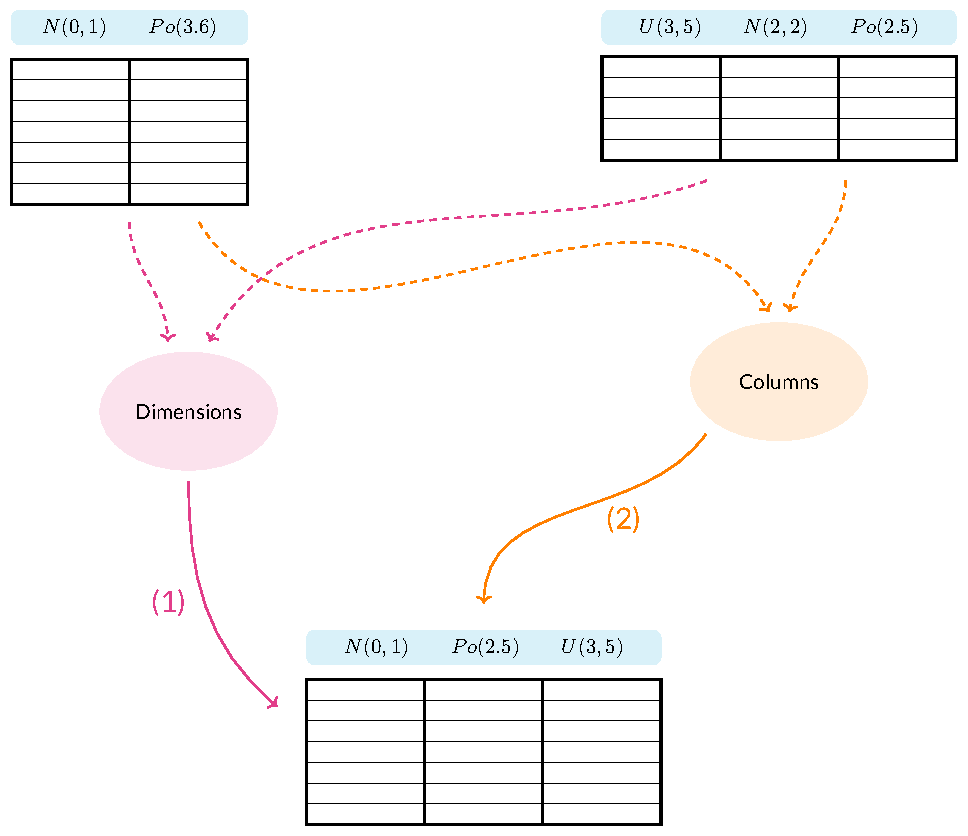
\includegraphics[width=.35\textwidth]{tex/crossover.pdf}
        \end{tabular}
    };

    \node (mut) at (30, -25) {%
        \begin{tabular}{c}
            \huge{Mutate offspring}\vspace{.5ex}\\
            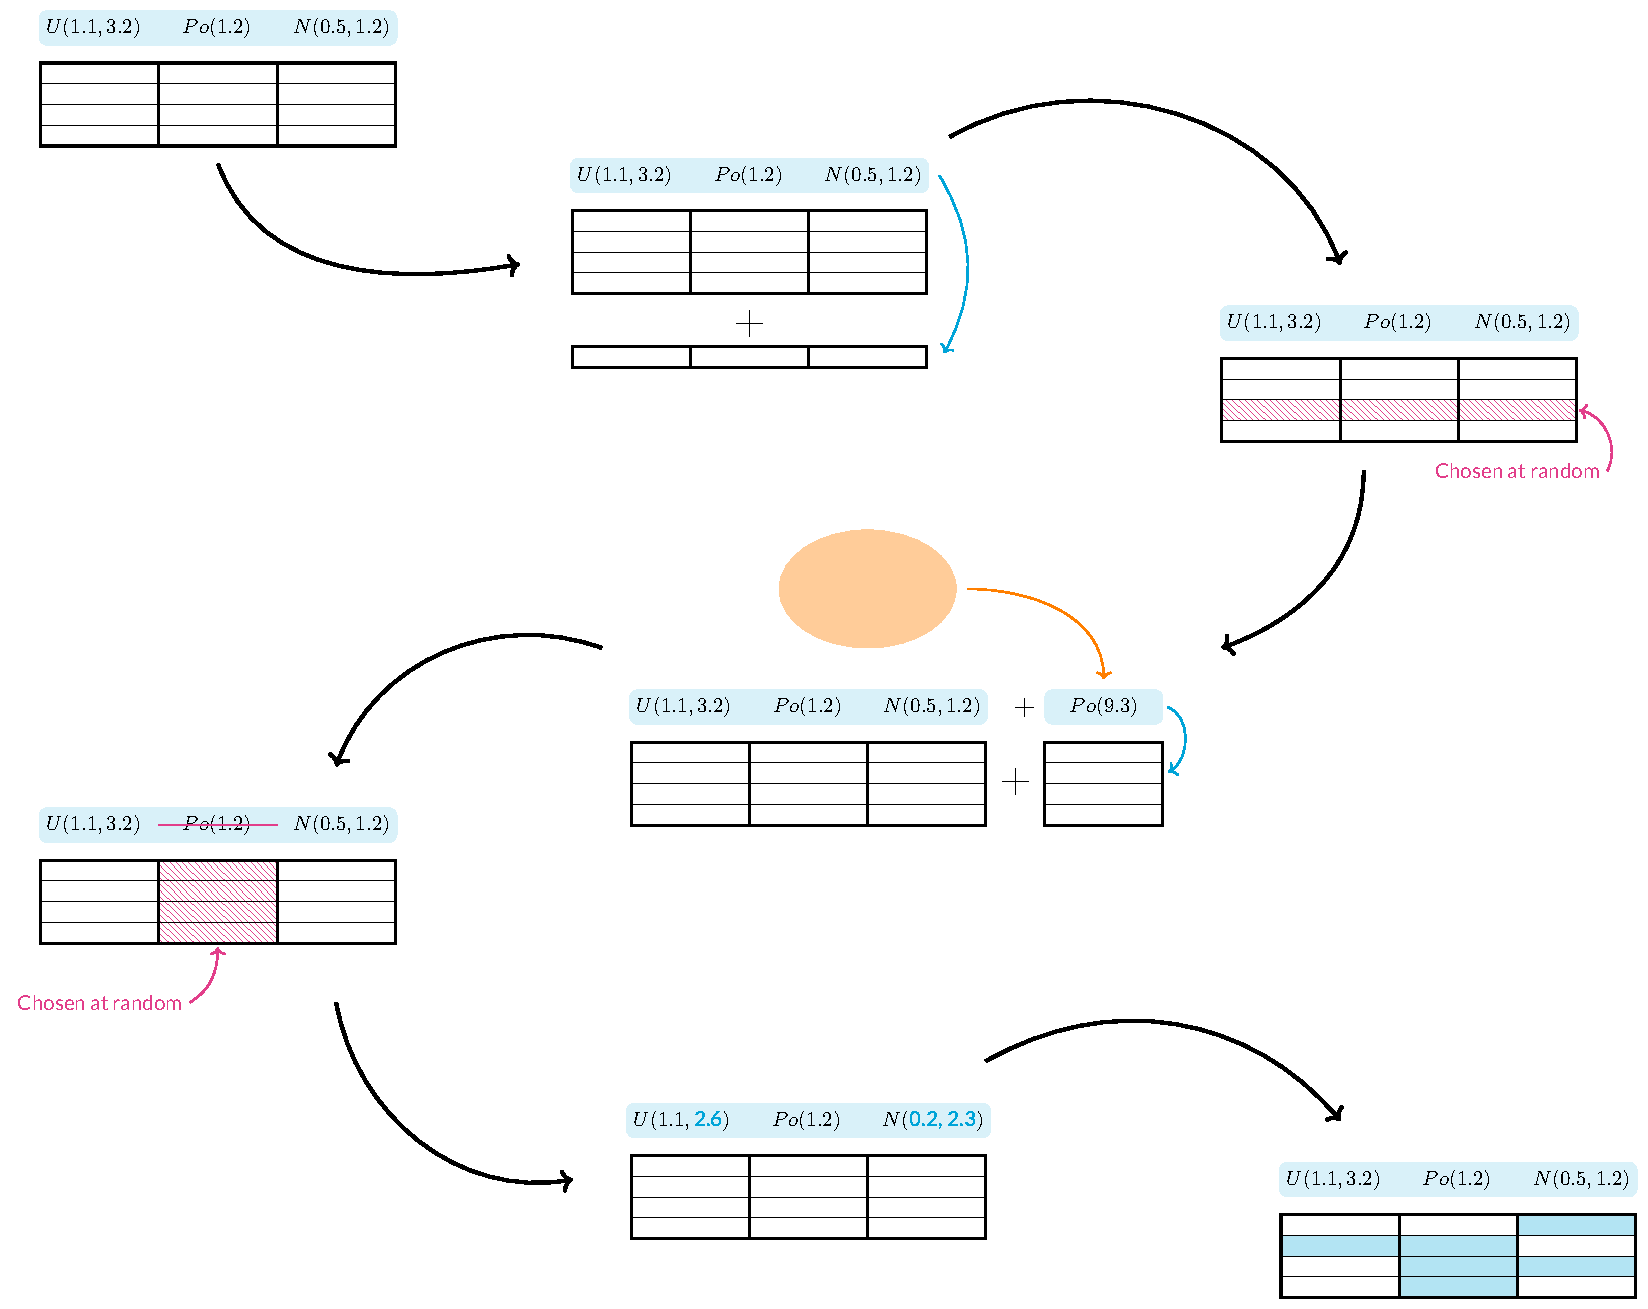
\includegraphics[width=.45\textwidth]{tex/mutation.pdf}
        \end{tabular}
    };

    \draw[->,myblue,line width=1ex] (ind.south) to[out=270,in=130] (sel.west);
    \draw[->,myblue,line width=1ex] ([xshift=4em] sel.north) to[out=90,in=200] (cro.west);
    \draw[->,myblue,line width=1ex] ([yshift=-3em] cro.east) to[out=300,in=90] (mut.north);
    \draw[->,myblue,line width=1ex] (mut.west) to[out=180,in=0] (sel.east); 

    \end{tikzpicture}
    \end{tcolorbox}

    \end{column}

    \begin{column}{0.3\textwidth}
        \begin{center}
            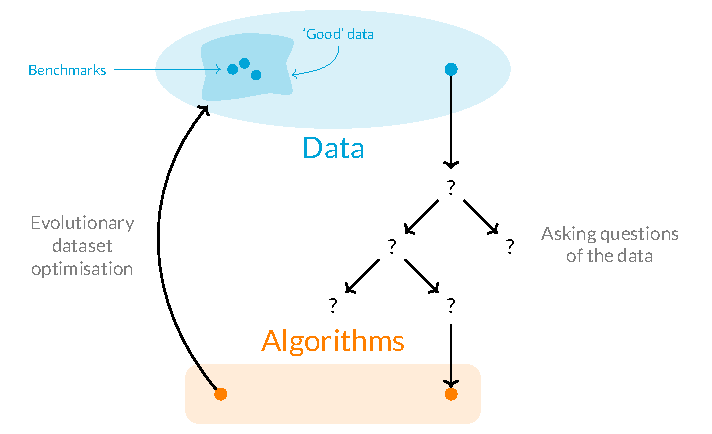
\includegraphics[width=\linewidth]{tex/paradigm.pdf}
        \end{center}

        \vfill%
        \begin{center}
            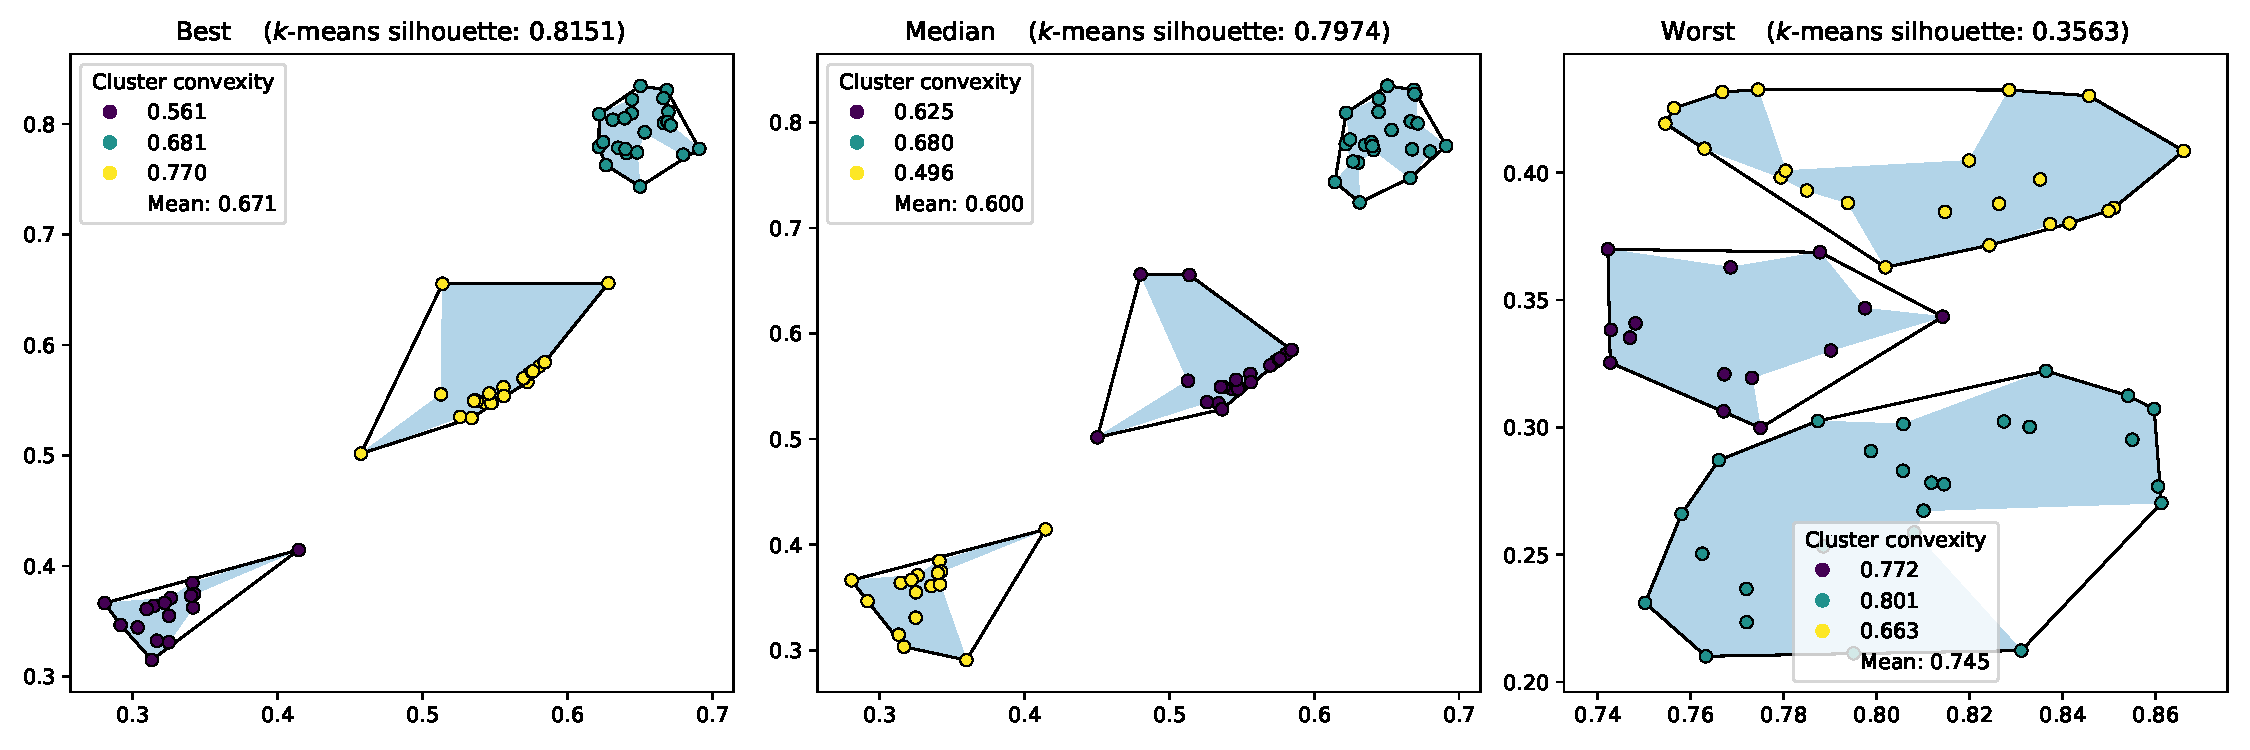
\includegraphics[width=\linewidth]{img/Fig12a.pdf}

            \vspace{1em}

            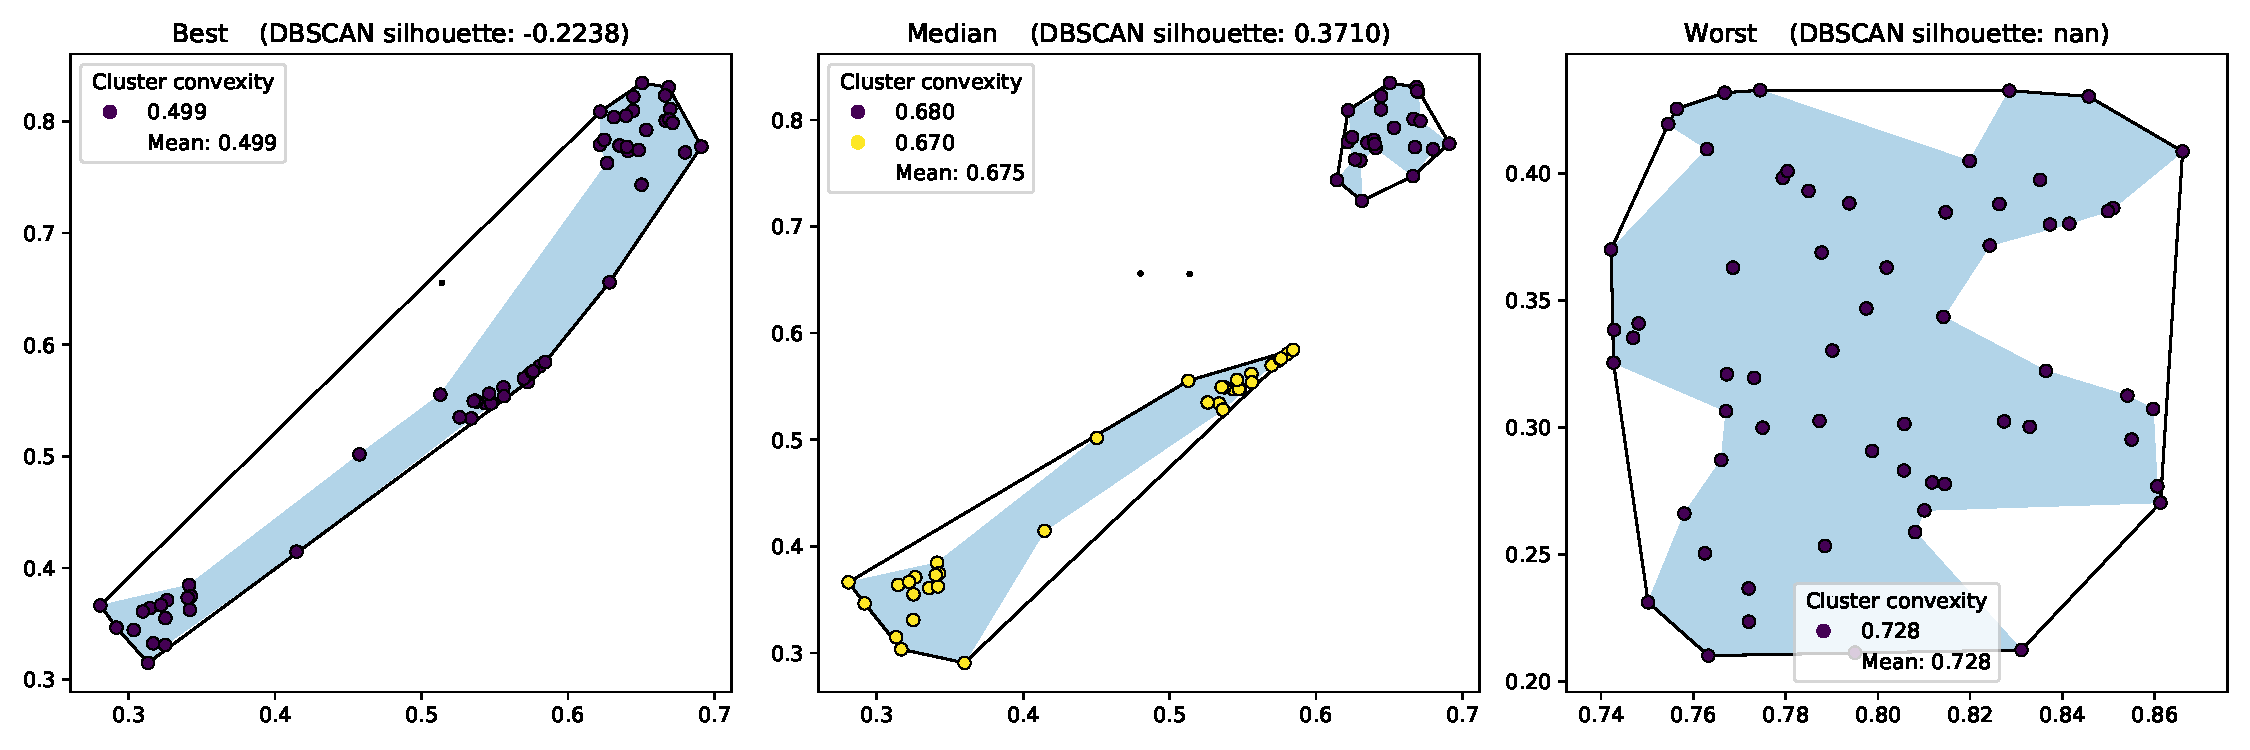
\includegraphics[width=\linewidth]{img/Fig12b.pdf}
        \end{center}
    \end{column}
\end{columns}

%%% FOOTER %%%

\vfill%
\begin{center}
    \huge{%
        \quad%
        \textbf{\faGithub~\faTwitter\quad daffidwilde}
        \hfill%
        \textbf{\faBook\quad \texttt{edo.readthedocs.io}}
        \hfill%
        \textbf{\faNewspaperO\quad \texttt{arxiv.org/abs/1907.13508}}
        \quad%
    }
\end{center}\vspace{1em}

\end{document}
